\problem{5}
{\sl Scaling of mean and fluctuation with system size.}
Divide a system into $m$ identical subsystems. For instance,
the diagram below shows a system being divided into $m=8$ subsystems.\par
\centerline{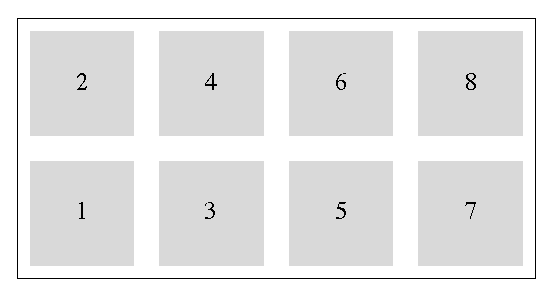
\includegraphics[width=0.4\textwidth,height=!]{subsystem}}\smallskip
\noindent Each subsystem $i$ has an internal energy $E_i$ that fluctuates over time.
The statistical average and variance, $\epsilon_i\equiv\ave{E_i}$ and
$\sigma^2_i \equiv \ave{(E_i - \ave{E_i})^2}$,
are identical for all subsystems.
So we discard the subscript $i$ and denote them by $\epsilon$ and $\sigma^2$.
For sufficiently large subsystems,
the effects of boundaries are negligible.
Write the total energy as a summation $E = \sum_{i=1}^m E_i$,
assume uncorrelated energy fluctuation in subsystems,
and show that the noise-to-signal ratio for $E$ scales as $1/\sqrt{m}$,
i.e.,
$$ \frac{\ave{(E - \ave{E})^2}^{1/2}}{\ave{E}} \propto \frac{1}{\sqrt{m}}\,, $$
which vanishes in the thermodynamic limit, $m\to\infty$.
This argument holds for all extensive quantities.

\bigskip\problem{10}
%{\sl Exercise~1.2 from David~Chandler, Introduction to Modern Statistical Mechanics.}
Two equations of state have been proposed for rubber bands (based on L.~R.G. Treloar's work, 1943):
$$ S = L_0 \gamma(\theta U/L_0)^{1/2} - L_0\gamma\left[
\frac{1}{2}\left(\frac{L}{L_0}\right)^2 + \frac{L_0}{L} - \frac{3}{2}\right],\qquad L_0=nl_0,$$
or
$$ S = L_0 \gamma\ee^{\theta n U/L_0} - L_0\gamma\left[
\frac{1}{2}\left(\frac{L}{L_0}\right)^2 + \frac{L_0}{L} - \frac{3}{2}\right],\qquad L_0=nl_0,$$
where $\gamma$, $l_0$, and $\theta$ are constants, $L$ is the length of the rubber band,
and the other symbols have their usual meaning: $S$ is entropy, $U$ is energy,
and $L_0 = n l_0$ is the rest length.

\smallskip
\subp Which of the two possibilities is acceptable? Why?

\smallskip
\subp
For the acceptable choice, find the expression for temperature $T$,
and deduce the dependence of the tension $f$ upon $T$ and $L/L_0$;
that is, deduce $f(T,L/L_0)$.
Here the tension $f$ is the force required to stretch the rubber band to length $L$.
%\hfil\break
{\bf Hint}: {\sl the first law is $dU = T dS + f d L$\/}.

\bigskip\problem{15}
{\sl Equation of state \& Legendre transform.}
The Helmholtz free energy for a fluid is given as
$$ F(N, V, T) = Nf_0 - Ns_0(T-T_0) - \frac{a N^2}{V} - NRT\ln\left(\frac{V/N-b}{v_0}\right)
+ N \int_{T_0}^T\left(\frac{T'-T}{T'}\right)c_v^\text{ideal}(T') \, dT' \,. $$
The notations have their standard meanings;
$f_0$, $s_0$, $T_0$, $a$, and $b$ are constants.

\smallskip\subp Find the internal energy expressed in terms of $N$, $V$ and $T$.

\smallskip\subp Find the mechanical equation of state, i.e., $PVT$ relationship, for this fluid.

\smallskip\subp Find the isothermal compressibility
$\kappa_T \equiv -\frac{1}{V}\pdc{V}{P}{T}$
and the (isobaric) thermal expansion coefficient $\alpha \equiv \frac{1}{V} \pdc{V}{T}{P}$.


